\section{Архитектура нейронной сети}
\subsection{Описание задачи и датасета}
В качестве примера возьмем нейронную сеть класификации цифр по картинке. За основу датасета возьмем MNIST датасет. В датасете педставлены чернобелые картинке рукописных цифр и соответсвующие им значения цифр, которые представлены на картинке. На каждом изображении изображена ровно одна цифра. Датасет разделен на 2 части: train и test для тестирования и обучения. Для практики выбрана такая задача, так как сеть для обучения получится легкой: в ней будет мало параметров, сеть обучается довольно быстро и за небольшое количество эпох, также данная задача хорошо подходит для исследования, так как на вход подается картинка, это пространство имеет размерность матрицы, на выходе же подается число, размерность которого одномерная. Соответственно в ходе преобразований сеть должна выявить все релевантные признаки и сильно сжать пространство, что полезно для нашего эксперимента.

\subsection{Архитектура сети}
Количество семплов в обучающей выборке 6000, размер каждого изображения (28, 28). Изображение одноканальное, так как оно чернобелое. Сеть предствляет собой следующую архитектуру
\begin{center}
    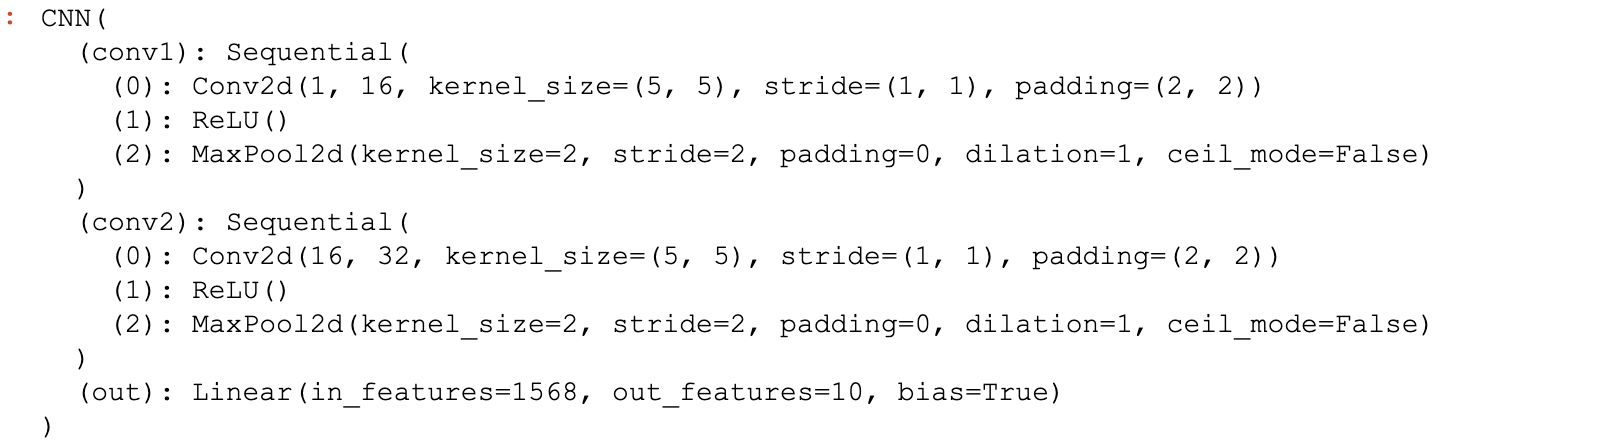
\includegraphics[scale=0.7]{images/CNN_arciticture.png}
\end{center}
Подробная количественная таблица параметров сети:
\begin{center}
    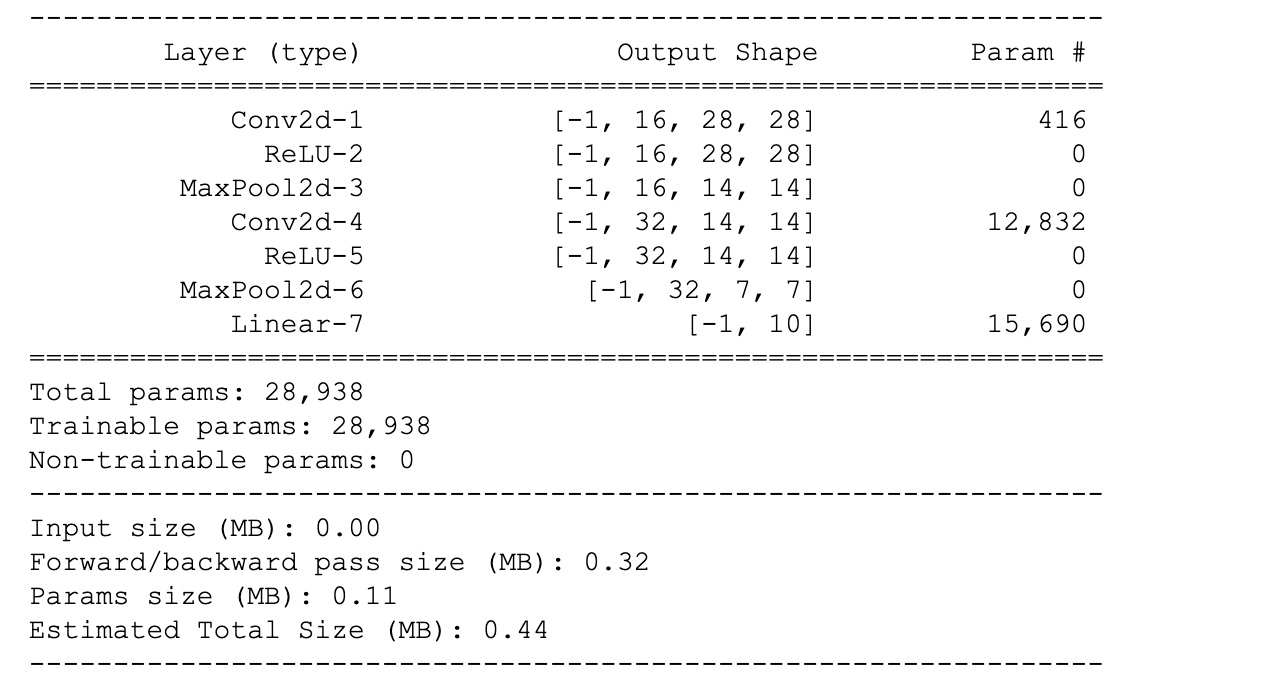
\includegraphics[scale=0.7]{images/cnn_params.png}
\end{center}
Соответственно сеть начинается с  2 сверточных слоев (conv1, conv2). Свертки представляют собой последовательность: 2d-свертка, функция архивации (ReLU()) и пуллинг (MaxPool2d). Далее после последововательных применений сверток conv1 и conv2 к входному тензору, тензор транспонируется в двумерный тензор, далее к нему применяется полнозвязный слой и функция Softmax. Финальное представление должно предсказывать вероятностное распределение на цифрах. \\
\subsection{Цикл обучения сети с подробным forward pass}
\begin{enumerate}
    \item $z_1 = conv1(x)$, где $x$ - входной батч, conv1 - первая свертка. $x.shape = (batch\_size, 1, 28, 28)$
    \item $z_2 = conv2(z_1)$, где $z_1$ - выход первого слоя сети, иначе говоря первого латентного пространства, conv2 - вторая свертка. $z_1.shape = (batch\_size, 16, 28 / 2, 28 / 2)  = (batch\_size, 16, 14, 14)$.
    \item $z_2^{flatten} = flatten(z_2)$, где $z_2$ - выход второго слоя сети, $flatten$ - функция меняющая размерность тензора, а именно превращая все признаки в одномерное векторное пространство. $z_2.shape = (batch\_size, 32, 14 / 2, 14 / 2) = (batch\_size, 32, 7, 7)$.
    \item $z_3 = linear(z_2^{flatten})$, где $z_2^{flatten}$ - выход второго одномерного слоя сети, $linear$ - полносвязный слой. $z_2^{flatten}.shape = (batch\_size, 32 * 7 * 7) = (batch\_size, 1568)$.
    \item $target = softmax(z_3)$, где $z_3$ - выход третьего слоя, функция softmax позволяет репрезентовать распределение, как вероятностное распределение в отрезке $[0, 1]$, $z_3.shape = (batch\_size, 10)$ 
    \begin{gather}
    \begin{aligned}
    softmax(x_i) = \exp(x_i) \setminus (\sum_{j}\exp(x_j))
    \end{aligned}
    \end{gather}
    \item Выход $y$ представляется как one hot вектор $y_{onehot}$, например 
    \begin{gather}
    \begin{aligned}
    y = 3 \Leftrightarrow y_{onehot} = [0, 0, 0, 1, 0, 0, 0, 0, 0, 0]
    \end{aligned}
    \end{gather}
    \item $y_{onehot}$ сравнивается с $target$ с помощью лосс функции кросс энтропии $L$
    \begin{gather}
    \begin{aligned}
    L(y, t) = - \sum_{i}y_i * \log(t_i)
    \end{aligned}
    \end{gather}
\end{enumerate}
Данная сеть обучалась с помощью инфмационной метрики в лоссе - кросс энтропии между таргетом и ground truth. При этом не учитывались никакие другие информационные эвристики в других латентных пространствах ($z_1, z_2, z_3)$.



